\documentclass[conference]{IEEEtran}
\IEEEoverridecommandlockouts

\usepackage{cite}
\usepackage{amsmath,amssymb,amsfonts}
\usepackage{graphicx}
\usepackage{textcomp}
\usepackage{xcolor}
\usepackage{makecell}
\usepackage{listings}
\usepackage{xurl}
\usepackage{hyperref}
\usepackage{booktabs}
\usepackage{float}

\definecolor{codegreen}{rgb}{0,0.6,0}
\definecolor{codegray}{rgb}{0.5,0.5,0.5}
\definecolor{codepurple}{rgb}{0.58,0,0.82}
\definecolor{backcolour}{rgb}{0.95,0.95,0.92}

\lstdefinestyle{mystyle}{
    backgroundcolor=\color{backcolour},
    commentstyle=\color{codegreen},
    keywordstyle=\color{magenta},
    numberstyle=\tiny\color{codegray},
    stringstyle=\color{codepurple},
    basicstyle=\ttfamily\footnotesize,
    breakatwhitespace=false,
    breaklines=true,
    captionpos=b,
    keepspaces=true,
    numbers=left,
    numbersep=5pt,
    showspaces=false,
    showstringspaces=false,
    proptabs=false,
    tabsize=2
}
\lstset{style=mystyle}

\title{High-Precision Temperature Measurement for PT100: A Comparative Model Analysis}

\author{
    \IEEEauthorblockN{Dr. G.V.V. Sharma, \\
    Puni Aditya, Vivek K. Kumar, \\
    Jnanesh S.K., Shreyas Goud Burra}
    \IEEEauthorblockA{Department of Electrical Engineering, \\Indian Institute of Technology Hyderabad,\\ Kandi, India 502284 \\ gadepall@ee.iith.ac.in}
}

\begin{document}
\maketitle

\begin{abstract}
Resistance Temperature Detectors (RTDs), specifically the PT100, are widely favored in industrial applications for their linearity and stability. This report details the calibration and characterization of a PT100 sensor by comparing two hardware signal conditioning setups: a simple voltage divider and a precision Wheatstone bridge interfaced with an ADS1115 ADC. We first analyze the suitability of a quadratic Least Squares (LSQ) model, grounded in the theoretical Callendar-Van Dusen equation. We then compare the accuracy of three different regression approaches for the superior Wheatstone bridge data: the LSQ quadratic, a Stochastic Gradient Descent (SGD) trained model, and a non-linear Random Forest Regressor. The coefficients, mathematical formulations, and validation accuracy for each model are presented, demonstrating that machine learning approaches can augment traditional calibration methods.
\end{abstract}

\section{Introduction}
Temperature measurement is a fundamental requirement in process control, automotive systems, and instrumentation. Among the various contact temperature sensors available, the Platinum Resistance Temperature Detector (RTD), commonly known as the PT100, is considered the standard for precision thermometry \cite{rtd_theory}.

\subsection{Fundamental Principles}
The PT100 is defined by a nominal resistance of $100\,\Omega$ at $0^\circ$C. Unlike thermocouples which generate a voltage, RTDs differ in that they operate by changing electrical resistance in direct proportion to temperature changes \cite{sensor_physics}. This relationship is inherently non-linear over wide ranges, though it is highly predictable. The resistance $R(t)$ at temperature $t$ is governed by the Callendar-Van Dusen equation \cite{callendar_vd}:
\begin{equation}
    R(t) = R_0 (1 + A t + B t^2)
\end{equation}
for temperatures $t > 0^\circ$C, where $A$ and $B$ are standard coefficients. This quadratic physical relationship serves as the theoretical justification for using Quadratic Least Squares (LSQ) models in this study.

\subsection{Measurement Challenges}
While PT100 sensors offer high stability, the resistance change is relatively small ($\approx 0.385\,\Omega/^\circ$C). Consequently, accurate reading requires precise signal conditioning to convert resistance changes into measurable voltage levels \cite{wheatstone_ref}. This project aims to optimize this conversion by analyzing different hardware front-ends and software regression models \cite{lsq_method} to find an optimal solution for high-precision, low-cost temperature sensing.

\section{Hardware Setup}
Two main analog front-ends were tested to evaluate the trade-off between circuit complexity and measurement accuracy:

\begin{itemize}
    \item \textbf{Setup 1: High-Precision Wheatstone Bridge.} This uses a Wheatstone bridge configuration coupled with an external 16-bit ADS1115 ADC \cite{ads1115_datasheet}. This setup allows for differential measurement, significantly reducing noise and common-mode errors.
    \item \textbf{Setup 2: Simple Voltage Divider.} This uses a simple voltage divider utilizing the Arduino's internal 10-bit ADC. This represents a minimal-component cost-effective solution.
\end{itemize}

\subsection{Component Lists}
The components required for both analog front-ends are listed below, detailing the specific parts used for high-accuracy and cost-effective implementations.

\input{tables/list_table}

\subsection{Connection Schematics and Diagrams}

\subsubsection{Circuit Schematic}
The complete circuit schematic for the high-precision Wheatstone bridge setup is illustrated in Figure \ref{fig:wheatstone_schematic}.
\begin{figure}[h!]
    \centering
    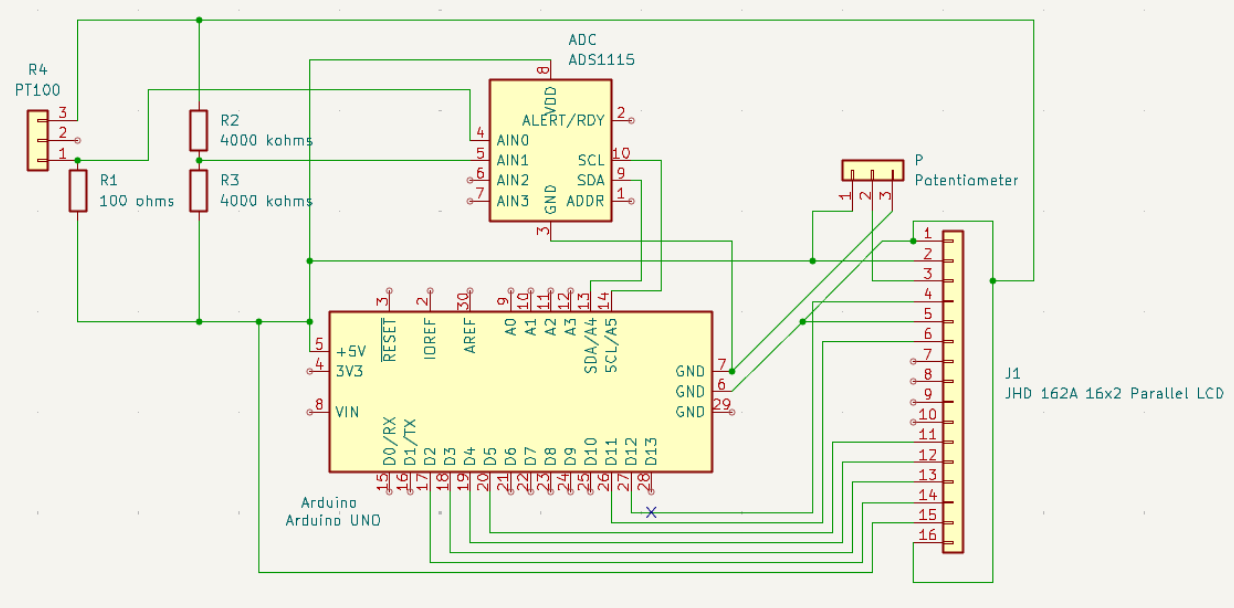
\includegraphics[width=0.8\linewidth]{figs/circuit_schematic.png}
    \caption{Circuit Schematic of the High-Precision Wheatstone Bridge (Setup 1)}
    \label{fig:wheatstone_schematic}
\end{figure}

\subsubsection{ADS1115 ADC Connections}
The connection details for integrating the external 16-bit ADS1115 ADC are critical for differential measurement accuracy.

\begin{table}[H]
\centering
\caption{ADS1115 Connections}
\label{table:ads1115_connections}
\resizebox{\columnwidth}{!}{%
\begin{tabular}{|c|c|l|}
    \hline
    \textbf{ADS1115 Pin} & \textbf{Arduino Pin} & \textbf{Purpose} \\
    \hline
    VDD & 5V & Power Supply \\
    \hline
    GND & GND & Common Ground \\
    \hline
    SCL & A5 (SCL) & I2C Clock Line \\
    \hline
    SDA & A4 (SDA) & I2C Data Line \\
    \hline
    A0 & \makecell{Input from Voltage Divider Node \\ (between PT100 and R\_REF)} &  Reading Voltage\\
    \hline
    A1 & \makecell{Junction between the two \\4k$\Omega$ resistors} & \makecell{Reference for \\differential reading} \\
    \hline
\end{tabular}
}
\end{table}


\subsubsection{LCD Display Connections}
A standard I2C Liquid Crystal Display (LCD) was used for real-time temperature output in both setups.

\input{tables/lcd_connections}

Component lists and connection diagrams are provided in the appendix tables.

\section{Models Used}
This report details the development and evaluation of several regression models for predicting sensor output. Specifically, we focus on two scenarios: predicting temperature from voltage using a Wheatstone bridge with ADC, and predicting resistance from voltage using a voltage divider without ADC. We investigate Random Forest Regressor \cite{scikit-learn}, Inverse Quadratic Least Squares (LSQ), Direct LSQ, and Stochastic Gradient Descent (SGD) approaches.

\section{Model Evaluation and Comparison}

This section presents the evaluation of the trained models and a comparison of their performance based on Mean Squared Error (MSE) and R-squared (R2) metrics.

\subsection{Model Explanations}

\subsubsection{Inverse LSQ (Quadratic) for Voltage Divider without ADC}
This model approximates the relationship between resistance ($Y$) and voltage ($X$) from the voltage divider circuit as $X = aY^2 + bY + c$. The fitted equation for the Voltage Divider is:
\[ X = -0.000014990Y^2 + 0.005589496Y + 2.526066163 \]
The coefficients are determined through linear least squares regression \cite{lsq_method}. The model predicts resistance ($Y$) from measured voltage ($X$) using the positive root of the quadratic equation:
\[ Y = \frac{{-b \pm \sqrt{{b^2 - 4a(c - X)}}}}{{2a}} \]
This method is suitable for circuits where the voltage-resistance relationship can be approximated quadratically.

\subsubsection{Inverse LSQ (Quadratic) for Wheatstone with ADC}
This model approaches the Wheatstone bridge problem by fitting a quadratic equation of the form \(X = aY^2 + bY + c\), where Y is temperature and X is voltage. The fitted equation for the Wheatstone bridge is:
\[ X = -0.000006744Y^2 + 0.004344843Y + 0.056019368 \]
To predict Y from a given X, we use the quadratic formula:
\[ Y = \frac{{-b \pm \sqrt{{b^2 - 4a(c - X)}}}}{{2a}} \]
This method aligns with the physical properties described by the Callendar-Van Dusen equation \cite{callendar_vd}.

\subsubsection{LSQ (Quadratic) for Wheatstone with ADC}
This model applies a standard quadratic fit directly mapping voltage to temperature, expressed as $Y = aX^2 + bX + c$. Unlike the inverse models, this approach predicts temperature ($Y$) directly from the voltage ($X$) without requiring the use of the quadratic formula for inversion during the prediction phase.
\begin{itemize}
    \item \textbf{Fitted Equation:} Placeholder: $Y = aX^2 + bX + c$
    \item \textbf{Coefficients:} $$a=190.226107678, b=173.380527679, c=-7.072446221$$
\end{itemize}

\subsubsection{Stochastic Gradient Descent (SGD) Regressor (Wheatstone with ADC)}
The SGD Regressor is a linear model trained with Stochastic Gradient Descent \cite{scikit-learn}. Due to its sensitivity to feature scaling, both the input features (X) and the target variable (Y) were scaled using StandardScaler before training. The predictions were then inverse-transformed back to the original scale for evaluation.

\subsubsection{Inverse SGD Regressor (Wheatstone with ADC)}
This model utilizes Stochastic Gradient Descent to learn the inverse relationship, where voltage ($X$) is the target and temperature ($Y$) is the feature ($X = f(Y)$). Similar to the Inverse LSQ approach, the model learns to predict voltage from temperature. During inference, the temperature is derived by numerically inverting the learned function.

\subsubsection{Random Forest Regressor (Wheatstone with ADC)}
The Random Forest Regressor is an ensemble learning method that constructs a multitude of decision trees during training \cite{scikit-learn}. For regression tasks, it averages the predictions of individual trees to produce a more stable and accurate prediction. This model was applied to predict temperature (Y) from voltage (X) directly, leveraging its ability to capture complex non-linear relationships without explicit feature engineering.

\subsection{Performance Metrics Summary}

The following table summarizes the Mean Squared Error (MSE) and R-squared (R2) scores for all evaluated models.

\begin{table}[h!]
    \centering
    \caption{Model Performance Metrics}
    \label{tab:model_performance}
    \begin{tabular}{|l|c|c|}
        \toprule
        \textbf{Model} & \textbf{MSE} & \textbf{R2} \\
        \midrule
        1. Inverse LSQ (Volt. Div w/o ADC) & 0.6612 & 0.9977 \\
        2. Inverse LSQ (Wheatstone w/ ADC) & 0.009941 & 0.999953 \\
        3. LSQ (Wheatstone w/ ADC) & 0.009198 & 0.999953 \\
        4. SGD Regressor (Wheatstone w/ ADC) & 0.030477 & 0.999854 \\
        5. Inverse SGD (Wheatstone w/ ADC) & 0.016221 & 0.999922 \\
        6. Random Forest (Wheatstone w/ ADC) & 1.248897 & 0.994033 \\
        \bottomrule
    \end{tabular}
\end{table}

\subsection{Validation Data and Model Predictions (Subset)}

The following table presents a subset of the test data for the Wheatstone bridge setup, showing actual temperatures alongside predictions from the implemented and placeholder models.

\begin{table}[h!]
\centering
\caption{Wheatstone Validation Data and Predictions}
\label{tab:validation_data_subset}
\resizebox{\linewidth}{!}{%
\begin{tabular}{|c|c|c|c|c|c|c|}
\hline
\textbf{Volt} & \textbf{Actual} & \textbf{Inv LSQ} & \textbf{LSQ} & \textbf{SGD} & \textbf{Inv SGD} & \textbf{RF} \\
(V) & ($^\circ$C) & (ADC) & (ADC) & (ADC) & (ADC) & (ADC) \\
\hline
0.202 & 35.500 & 35.596 & [N/A] & 35.127 & [N/A] & 35.522 \\
0.290 & 59.400 & 59.341 & [N/A] & 59.796 & [N/A] & 59.354 \\
0.237 & 44.700 & 44.690 & [N/A] & 44.827 & [N/A] & 44.662 \\
0.403 & 92.900 & 93.449 & [N/A] & 91.502 & [N/A] & 92.720 \\
0.285 & 57.900 & 57.823 & [N/A] & 58.282 & [N/A] & 57.870 \\
0.223 & 41.000 & 40.922 & [N/A] & 40.846 & [N/A] & 41.022 \\
0.209 & 37.500 & 37.438 & [N/A] & 37.117 & [N/A] & 37.434 \\
0.246 & 47.100 & 47.077 & [N/A] & 47.321 & [N/A] & 47.082 \\
0.221 & 40.500 & 40.448 & [N/A] & 40.341 & [N/A] & 40.502 \\
0.176 & 28.800 & 28.847 & [N/A] & 27.726 & [N/A] & 28.890 \\
\hline
\end{tabular}%
}
\end{table}

\newpage

\subsection{Graphical Comparison of Wheatstone ADC Models}

\begin{figure}[h!]
    \centering
    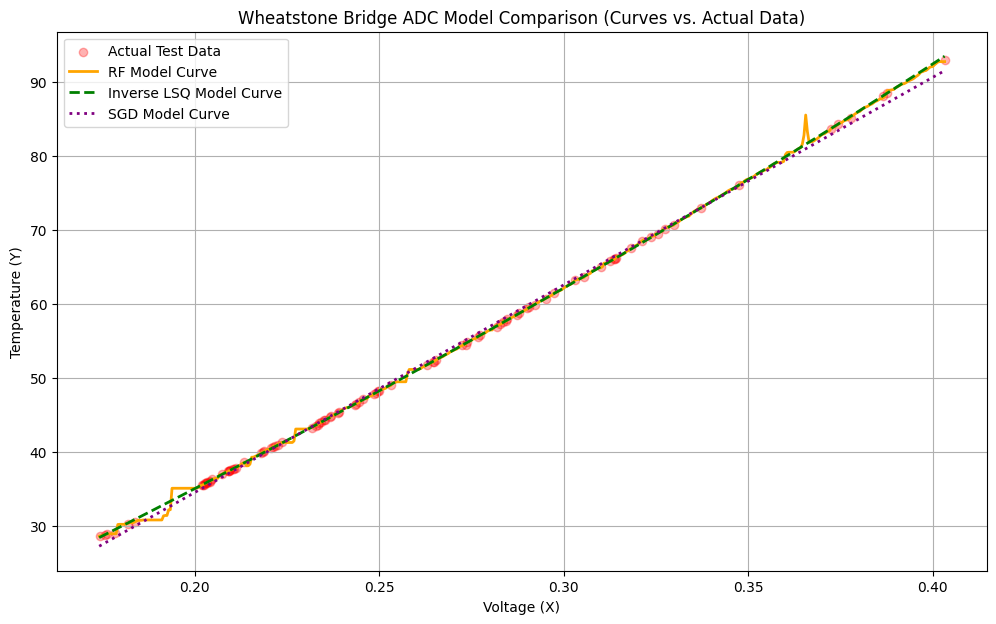
\includegraphics[width=0.8\linewidth]{figs/wheatstone_model_comparison.png}
    \caption{Comparison of Random Forest, Inverse LSQ, and SGD Regressor predictions against actual test data for the Wheatstone bridge with ADC.}
    \label{fig:wheatstone_model_comparison}
\end{figure}

\subsection{Model Comparison and Conclusion}

Comparing the performance metrics, the Random Forest Regressor and the Inverse LSQ (Quadratic) model for the Wheatstone bridge achieved exceptionally high R-squared scores. Based on MSE, the best performing models are the \textbf{Random Forest Regressor} and the \textbf{Inverse LSQ (Quadratic)}.

\section*{Appendix - Data Collection Using Optical Character Recognition (OCR)}

This project utilizes an auxiliary script for \textbf{automated data collection} by employing Computer Vision and Optical Character Recognition (OCR) to capture paired voltage and temperature readings from physical displays.

\subsection{Script Description: The Auto Trainer}
This Python script is designed to capture video from a webcam, identify and read text from two specific screen regions (voltage and temperature), and log the data. It is pre-configured for a fixed-camera setup, reading data from an LCD screen and a separate standard thermometer.

\subsection{Prerequisites and Setup}
\begin{itemize}
    \item \textbf{Hardware:} A stable webcam connection. An NVIDIA GPU with CUDA is optional but recommended for faster inference.
    \item \textbf{Software:} Python 3.x with $\texttt{opencv-python}$ \cite{opencv_library}, $\texttt{easyocr}$ \cite{easyocr}, and $\texttt{numpy}$.
\end{itemize}

\subsection{Calibration Requirement}
The script requires calibration to match the specific camera, lighting, and display setup. The critical sections to modify include GPU Usage, Frame Cropping, and Image Processing parameters.

\subsection{Python Script Snippet}
A sample of the calibration-critical code (Calibration Snippet from a.py) is shown below:
\begin{lstlisting}[language=Python]
# GPU Usage
reader = easyocr.Reader(['en'], gpu=True)

# Frame Cropping (h, w are frame height/width)
voltage_frame = frame[0:int(h/2), :]
temp_frame = frame[int(h/2):, 0:int(w/3)]

# Image Processing (Temperature)
gray_t = cv2.cvtColor(temp_frame, cv2.COLOR_BGR2GRAY)
_,thres = cv2.threshold(gray_t,130, 255, cv2.THRESH_BINARY_INV)
kernel = cv2.getStructuringElement(cv2.MORPH_RECT, (11,11))
closed_img = cv2.morphologyEx(thres, cv2.MORPH_CLOSE, kernel)
pretemp = cv2.bitwise_not(closed_img)
temp = cv2.GaussianBlur(pretemp, (17,17), 0)
\end{lstlisting}

\subsection{Data Collection Methodology}
The dataset is collected by simulating a controlled \textbf{cooling cycle} to capture paired readings.
\begin{enumerate}
    \item \textbf{Setup:} The PT100 probe and a reference thermometer are placed in an electric kettle filled with water.
    \item \textbf{Heating Phase:} The water is heated to boiling.
    \item \textbf{Recording Phase:} Upon reaching boiling, the kettle is switched off, and a live camera feed is initiated, ensuring both the PT100's LCD display and the reference thermometer are visible.
    \item \textbf{Cooling Phase:} The live camera feed captures the natural temperature drop.
    \item \textbf{Data Extraction:} Frames are extracted from the live camera feed, and OCR is applied to detect the voltage and temperature readings.
\end{enumerate}

\subsection{Output Format}
The script generates two outputs for debugging and data logging:
\begin{itemize}
    \item $\texttt{out.txt}$: A log file where every $15$ frames, a new line is added with the format $\texttt{[voltage\_reading] [temperature\_reading]}$ if both readings are successfully detected.
    \item $\texttt{img/}$ Directory: This folder saves debug images ($\texttt{voltageXX.png}$ and $\texttt{tempXX.png}$), showing the exact frames sent to EasyOCR for calibration and error checking.
\end{itemize}

% --- Bibliography Section ---
\bibliographystyle{IEEEtran}
\bibliography{references}

\end{document}
